\hypertarget{paper-2}{%
\chapter{Information-Seeking Behaviors for Information on Covid-19 Vaccinations}\label{paper-2}}

\hypertarget{abstract}{%
\section{Abstract}\label{abstract}}

Previous research has greatly failed to distinguish between the activation of
information seeking behaviors online and offline. Using theories of social
support and uses and gratifications theory I investigate the factors associated
with each vehicle type when on information seeking vehicle: personal connection,
doctor, social networking site, online forum, and online search engine. Using
novel survey data of 948 Americans and their experience seeking out
information about the Covid-19 vaccines, I find little evidence that online
search is more utilized than seeking social support from personal network
connections or health professionals. I find evidence that the vehicles queried
in this survey are conceptually different and that the utilization of different
vehicles varies by demography and information sources. Finally, I find that
different fountains of information and information search vehicles hold real
world consequences through their associations with Covid-19 vaccination rates
and intentions, as information from a doctor increased the Covid-19 vaccination
uptake while receiving information from a Social Networking Site like Facebook
or Twitter was associated with lower odds of vaccination.

\textbf{Keywords}: Information-Seeking Behavior, Covid-19, Vaccine Hesitancy, Social Networks, Social Support, Information \& Communication Technologies

\hypertarget{intro-1}{%
\section{Intro}\label{intro-1}}

Information is all around us and permeates every facet of human society, from
the hordes of data gathered during the internet age or passing gossip between
friends. Human communication and human society are based on the circulation of
information and knowledge. Information can be shared by others through
information campaigns and consumed by an individual, called information push, or
intentionally sought out by individuals, called information pull
\citep{cybenkoFoundationsInformationPush1999}.

Information is especially important given the prominent trends of
misinformation, disinformation, and mistrust in traditional institutions
\citep{starbird19, kata10}. While no belief in false information can be thought of as
harmless \citep{douglas21} some discredited theories such as 'vaccines cause autism'
have major ramifications for both the individual and the social world that
surrounds them. For example, a newfound public resistance to vaccination
against Measles by so-called 'anti-vaxxers' caused a 17\% increase in rates
worldwide in 2019. This increase killed  142,000 people, most of whom were
children under the age of five \citep{givetash19}. However, even in the ever-evolving
research agenda of misinformation and infodemiology \citep{eysenbach02}, much of the
research focuses on the 'push' or 'supply' side of information, like spaces where
individuals first encounter with conspiracy theories or other information
\citep{johnsonOnlineCompetitionPro2020, broniatowski_etal20}.
% cite something else here 

The lack of research in which vehicles are likely to be chosen when an
individual faces a need for information makes it difficult for policy makers to
propose effective information campaigns that promote the health and wellbeing of
individuals in our society. Even outside of the misinformation literature, much
of the research conducted in social networks and communication focus on senders,
influencers, and persuasion strategies 
\citep{mertonManifestLatentFunctions1968, katzPersonalInfluencePart1955, lazarsfeldPeopleChoice1944},
rather than on
“the receiver as an active information seeker and processor." \citep{johnsonComprehensiveModelCancerRelated1993},
though there are always exceptions \citep{eysenbach09}

I use the case of information around Covid-19 vaccinations to explore the
variation of usage of information search vehicles. In doing so, I seek to answer
how computer-mediated or interpersonal information-seeking strategies vary
across populations in their search for information about Covid-19 vaccinations
and investigate how these strategies affect vaccination uptake.

Before addressing my central research questions, I offer an overview of the
current state of social science literature in regards to information-seeking
strategies before providing a description of the research methodology and
analytic sample. I discuss the implications of these findings for the
sociological understanding of information search and vaccination uptake.

\hypertarget{information-search}{%
\subsection{Information Search}\label{information-search}}

Active, directed searching by individuals to obtain information is sparsely
discussed in the sociological literature. Pejtersen \citet{pejtersenDesignComputeraidedUsersystem1984}, a scholar
of library and information science, theorized that there are 5 strategies for
searching for information. The most common strategy is browsing, where people
follow leads based on associations without premeditation. Another strategy is
analytical, which includes an explicit consideration of all facets of the
question to guide a search. The empirical method guides the search based on
tactics that were successful in past research. The known site strategy is to go
to the direct source of the information if known. And finally, the similarity
method is to find information based on another similar question that already has
an answer. These 5 strategies vary in their demands for prior knowledge,
cognitive processing, memory, and time spent. While this theory is aimed at
finding information in a library setting, scholars have extended the theory to
other fields and validated the framework
\citep{fidelHumanInformationInteraction2012}; the frame is a useful beginning point
for my theories of information search through network activation or through
computer-mediated communication.

Some communication theorists ask why an answer to a question is sought in the
first place. The Theory of Uncertainty Management
\citep{brashersCommunicationUncertaintyManagement2001} professes that people search
for information when their uncertainty around the subject leads to anxiety or
other cognitive harms. The Theory of Motivated Information Management
\citep{afifiTheoryMotivatedInformation2004, afifiSeekingInformationSexual2006}
extends the prior by adding that uncertainty itself is not the catalyst for
information-search; rather, it is driven by a discrepancy between the current
level of uncertainty on a subject and desired level of uncertainty. In other
words, individuals only perform information search when they are distressed by
their lack of knowledge or understanding on a subject.

One way to find information is to activate network ties to find out information
through a form of social support. Social support, while previously used
interchangeably with the term social networks and social integration
\citep{houseStructuresProcessesSocial1988}, are the emotional, informational, and
instrumental assistance functions performed between social ties and have strong
and measurable association with health outcomes
\citep{houseMeasuresConceptsSocial1985, thoitsMechanismsLinkingSocial2011}.
Informational support is the process of seeking “help in defining,
understanding, and coping with problematic events and include education, advice,
or referral to another source of support” \citep{winemiller_etal93}[p. 640].
Brashers, a health communications researcher, defines informational support
slightly differently, focusing on the exchange of information that “facilitates
coping with life stresses… that may be exchanged among members of a support
network” \citet{brashersInformationSeekingAvoiding2002}[p. 260].These definitions
help to differentiate between seeking information through social ties or through
something anonymous like online search; a need for coping or deeper
understanding of important matters is thought to sway that decision.

Social support has long been theorized to stem from core discussion networks and
much of the historical social support surveys only looked at these core
networks. The underlying assumption is that individuals reach out to a handful
of strong ties when in need of support, which could be elicited in surveys using
name generators \citep{marsdenCoreDiscussionNetworks1987}. This approach has yielded
important insights, but largely overlooks crucial
processes of resource activation \citep{hurlbertCoreNetworksTie2000,
perrySocialNetworkActivation2015, smithDonPutMy2005}. For instance, Small
\citet{smallSomeoneTalk2017} shows that the core discussion network does not capture
how people activate social support in practice and indicates that people draw on
much broader social connections for support, reminiscent of the weak ties
research by Granovetter \citet{granovetterStrengthWeakTies1973}. There is ongoing
research investigating how weak-tie support holds for different support types
based on the architecture put forward by 
\citet{houseStructuresProcessesSocial1988} of instrumental, emotional, and
informational support. 

However, informational support can also be sought outside of the social network
context, namely via computer-mediated information search tools such as the
process of “Googling”. As the online environment began penetrating all facets of
modern human life, it makes sense that performing online search has become one
of the most convenient vehicles for information search. While Small
\citet{smallSomeoneTalk2017} focuses on how support can depend on a network tie
simply "happened to be there", online search is theoretically the most
frictionless and costless mode of support. No social capital or relationship is
necessary when choosing to utilize a search engine. 

There are three computer-mediated vehicles I consider for this analysis: online
search engines like Google or Bing, posting questions on online forums like
subreddits or Facebook groups, and posting a status update online via Facebook
or Twitter. While the first two are largely anonymous and don't require a
personal network, the third is a unique hybrid between personal network
connections and online search.

There are important factors that can influence information-seeking strategies
besides the strength of social capital or ease of search. For instance, we can
borrow uses and gratifications theory (UGT) from studies of mass communication
\citep{blumlerUsesMassCommunications1974, tanMassCommunicationTheories1985}
. UGT
posits that users are not passive consumers of media and that people have an
active role in choosing different sources of media based on their satisfaction
of specific needs on an individual basis. UGT is based on Maslow’s  \citeyear{maslowTheoryHumanMotivation1943} hierarchy of needs and is compatible with
Lazarsfeld and Katz’s theory of two-step flow \cite{katzPersonalInfluencePart1955}
because people can choose their media and the opinion leaders they follow.
Modern-day theorists have extended UGT theory and classified the uses and
gratifications of the internet and of social media. \citet{staffordDeterminingUsesGratifications2004} theorize that the internet
provides gratification through useful content that meets expectations,
gratification from purposeful navigating or random browsing as a process, and
social gratification from forming and deepening social ties. \citet{leungGenerationalDifferencesContent2013} theorizes that social media is
gratifying for users because it allows for venting of negative feelings,
provides recognition, provides entertainment, promotes social affection, and
fulfills cognitive needs. 

Adapting these facets of UGT and social support to my own case, I theorize that
online search allows for increased anonymity, a lowered social cost, and the
potential avoidance of embarrassment and other negative social interactions,
especially in the case on search engines. \citet{rainsCopingIllnessDigitally2018}
finds that patients tend to search for
technical information about an illness online but they then turn to their social
network for experiential information from others facing similar circumstances in
the case of cancer. The type of information sought is therefore important.
If specific expertise on a specific topic is desired by a searcher, they may
reach out to personal connections that they see as expert such as a doctor, or
if an individual distrusts the medical establishment, they may be more likely to
activate informational support among their social network or turn to online
groups that validate their worldview \citep{bogersHowSocialAre2014}. Finally, UGT and
Brasher's definition of social support \citeyearpar{brashersInformationSeekingAvoiding2002} help us to theorize that the
psychosocial needs like identity management or relational maintenance of an individual may influence their chosen information search vehicle: when the informational need is related to
forming and deepening social ties search is likely to be done from network ties.

\hypertarget{research-methodology}{%
\section{Research Methodology}\label{research-methodology}}

The data used for this research project are based on original survey data
sampled between December 03, 2021 through
December 12, 2021. This survey was hosted on Qualtrics and
participants were paid and recruited using Amazon Turk (MTurk). The total valid
survey responses (\emph{n} = 948) were selected from a total of 1,066
respondents; some responses were disqualified due to a few factors such as
detected usage of a VPN, random answer clicking (determined by illogical
responses), poor quality typed responses (e.g., social network alters
consistently named random nouns), or taking the survey more than once. The same
is slighted gender unbalanced, slightly skewing towards a male sample. For the
respondents who provided their zip code (p = 0.98), the sample is quite balanced with a slight skew towards MTurkers in the South (p = 0.41).

The survey took an average of 24.48 minutes with a standard deviation of 13.23 minutes. The shortest valid survey took 3.75 minutes and the longest took 111.08 minutes. Participants were paid \$6.00 for their time after Amazon administrative fees, funded by a Grant awarded to Kelsey E. Gonzalez and Nicolas Legewie by the Summer Institute in Computational Social
Science and the Russell Sage Foundation. The main portion of this survey replicates the book, Someone to Talk To \citep{smallSomeoneTalk2017} by expanding on Small's finding that people draw on much broader sources than ``important people'' for support by segregating weak-tie social support into instrumental, emotional, and informational support \citep[see][]{houseStructuresProcessesSocial1988}. The latter
part of the survey focuses on resource activation for the specific case-study of
information during the Covid-19 pandemic analyzed in this paper.

\begin{table}[ht]

\caption{\label{tab:table-1-desc}Descriptive Statistics for Dichotomous and Numeric Variables}
\centering
\begin{tabular}{lrr}
\toprule
  & Mean & SD\\
\midrule
Received info & \num{0.66} & \num{0.47}\\
Received info, Doctor & \num{0.47} & \num{0.50}\\
Received info, Person & \num{0.67} & \num{0.47}\\
Received info, News & \num{0.65} & \num{0.48}\\
Received info, Social Networking Site & \num{0.40} & \num{0.49}\\
Received info, Online Forum & \num{0.35} & \num{0.48}\\
Sought Info & \num{0.78} & \num{0.41}\\
Sought Info, Doctor & \num{0.44} & \num{0.50}\\
Sought Info, Person & \num{0.42} & \num{0.49}\\
Sought Info, Social Networking Site & \num{0.18} & \num{0.39}\\
Sought Info, Online Forum & \num{0.27} & \num{0.44}\\
Sought Info, Online Search & \num{0.41} & \num{0.49}\\
Vaccination Status & \num{0.84} & \num{0.36}\\
Vaccination Outlook & \num{0.87} & \num{0.34}\\
Age & \num{37.76} & \num{10.75}\\
Hispanic or Latino/x & \num{0.15} & \num{0.36}\\
Race, White & \num{0.88} & \num{0.33}\\
Race, Black & \num{0.08} & \num{0.27}\\
Race, Native American & \num{0.03} & \num{0.16}\\
Race, Asian or Pacific Islander & \num{0.04} & \num{0.20}\\
Associate's Deg or above & \num{0.74} & \num{0.44}\\
\bottomrule
\multicolumn{3}{l}{\rule{0pt}{1em}Notes: 948 Surveyed, Conducted December 03 through December 12, 2021.}\\
\end{tabular}
\end{table}

\hypertarget{measures}{%
\subsection{Measures}\label{measures}}

\hypertarget{sought-information}{%
\subsubsection{Sought Information}\label{sought-information}}

There are multiple dependent variables of interest for this paper. The first
variable is a dichotomous indicator of whether someone intentionally sought out
information about Covid-19 vaccinations. The survey asked, ``And how about you
yourself intentionally looking for information about a Covid-19 vaccine? Such
information can include things such as advice, clarification, facts, and
experiences.'' About 78\% (\(\widehat{p}\))
of respondents had intentionally sought out information about Covid-19
vaccinations (95\% Confidence Interval = \{76\%, 81\%\}).

Further dependent variables segment the above question into multiple options;
``How did you look for information about the Covid-19 vaccine?'' Respondents were
posed with 5 responses and `other,' of which they could select multiple. The
largest proportion, 44\%, asked their `doctor or another health professional' (95\% Confidence Interval = \{41\%, 47\%\}). About 42\% said they asked, `a person
like friend, neighbor, or family member that {[}they{]} know' (95\% Confidence
Interval = \{39\%, 45\%\}). An additional 41\% searched `for {[}their{]} question
using an online search engine such as Google or Bing' (95\% Confidence Interval
= \{38\%, 45\%\}). About a quarter of the sample, 27\%, `posted queries in an
online discussion group, listserve, or other online forum like a Facebook Group
or Subreddit' (95\% Confidence Interval = \{24\%, 30\%\}). And finally, 18\% of the sample `posted queries on a social networking site such as Facebook timeline, Twitter status update, or LinkedIn' (95\% Confidence Interval = \{16\%, 21\%\}).
Much of the question wording and the specific categories of search were inspired
by ICPSR project 37220 \citep{scanlon19}.

\begin{table}[!h]

\caption{\label{tab:table-2-desc}Descriptive Statistics for Categorical Variables}
\centering
\begin{tabular}[t]{llrr}
\toprule
  &    & N & Percent\\
\midrule
\cellcolor{gray!6}{Gender} & \cellcolor{gray!6}{Female} & \cellcolor{gray!6}{418} & \cellcolor{gray!6}{\num{44.09}}\\
 & Male & 524 & \num{55.27}\\
\cellcolor{gray!6}{} & \cellcolor{gray!6}{Other} & \cellcolor{gray!6}{6} & \cellcolor{gray!6}{\num{0.63}}\\
Highest Education Level & Graduate or professional degree & 145 & \num{15.30}\\
\cellcolor{gray!6}{} & \cellcolor{gray!6}{Bachelor's degree} & \cellcolor{gray!6}{560} & \cellcolor{gray!6}{\num{59.07}}\\
 & Associate's or Technical degree & 72 & \num{7.59}\\
\cellcolor{gray!6}{} & \cellcolor{gray!6}{Some college} & \cellcolor{gray!6}{100} & \cellcolor{gray!6}{\num{10.55}}\\
 & High school graduate & 68 & \num{7.17}\\
\cellcolor{gray!6}{} & \cellcolor{gray!6}{Less than high school} & \cellcolor{gray!6}{3} & \cellcolor{gray!6}{\num{0.32}}\\
Plan to be Vaccinated if not & Probably not & 38 & \num{4.01}\\
\cellcolor{gray!6}{} & \cellcolor{gray!6}{Definitely yes} & \cellcolor{gray!6}{13} & \cellcolor{gray!6}{\num{1.37}}\\
 & Definitely not & 61 & \num{6.43}\\
\cellcolor{gray!6}{} & \cellcolor{gray!6}{Might or might not} & \cellcolor{gray!6}{22} & \cellcolor{gray!6}{\num{2.32}}\\
 & Probably yes & 13 & \num{1.37}\\
\cellcolor{gray!6}{Found Info Sought Useful} & \cellcolor{gray!6}{Very useful} & \cellcolor{gray!6}{345} & \cellcolor{gray!6}{\num{36.39}}\\
 & Moderately useful & 112 & \num{11.81}\\
\cellcolor{gray!6}{} & \cellcolor{gray!6}{Extremely useful} & \cellcolor{gray!6}{264} & \cellcolor{gray!6}{\num{27.85}}\\
 & Slightly useful & 18 & \num{1.90}\\
\cellcolor{gray!6}{} & \cellcolor{gray!6}{Not at all useful} & \cellcolor{gray!6}{2} & \cellcolor{gray!6}{\num{0.21}}\\
Census Region & Midwest & 171 & \num{18.04}\\
\cellcolor{gray!6}{} & \cellcolor{gray!6}{Northeast} & \cellcolor{gray!6}{170} & \cellcolor{gray!6}{\num{17.93}}\\
 & South & 365 & \num{38.50}\\
\cellcolor{gray!6}{} & \cellcolor{gray!6}{West} & \cellcolor{gray!6}{223} & \cellcolor{gray!6}{\num{23.52}}\\
\bottomrule
\multicolumn{4}{l}{\rule{0pt}{1em}Notes: 948 Surveyed, Conducted December 03 through December 12, 2021.}\\
\end{tabular}
\end{table}

\hypertarget{vaccination-outlook}{%
\subsubsection{Vaccination Outlook}\label{vaccination-outlook}}

Another Dependent variable for this analysis is a dichotomous variable
indicating whether the respondent has received or plans to receive a vaccination against Covid-19. For this survey, the number of doses or timeline of receipt were less
relevant to the research question. This variable instead focuses on intent or
opinion about the vaccine. About 87\% have a
positive view about the vaccine. This construct is made through the combination
of two survey items. The first item is actual vaccination status, obtained through
the question `Did you receive a Covid-19 vaccine?'
84\% of the sample said that
they had indeed received a vaccination (95\% Confidence Interval = \{82\%, 87\%\}). As the national vaccination rate is closer to 75\% \citep{cdc20}, this indicates some bias in our sample that must be
acknowledged: either MTurkers are more likely to be vaccinated that the normal
population (sampling bias) or there is some conformity bias in the responses
causing survey takers to provide false answers. The second survey item that
contributes to `Vaccination Outlook' was only given to those who had not
responded `yes' to the to their vaccination status. These respondents were asked `Do you
plan to receive a vaccine for the prevention of the Covid-19 virus?' Of those
who were asked this question (n = 147), 9\% said they were `definitely yes' getting the vaccine;
9\% said they were `probably yes' going to receive vaccine. The rest of the sample was more unsure: 15\% said they `Might or might not,' 26\% said `Probably not,' and finally 41\% said they would `definitely not' receive the vaccine. The variable `Vaccination Outlook' indicates that either the respondent received a Covid-19 vaccine or
either probably or definitely will in the future.

\hypertarget{independent-variables}{%
\subsubsection{Independent Variables}\label{independent-variables}}

The first independent variables used in this analysis are based on the question,
`In the past 12 months, without searching for it, did you receive information
about the Covid-19 vaccine from \ldots{} (check all sources you received information
from).' This differs from the `How did you look for information' question above
because this is based on passive reception of information. The largest proportion
of respondents had received information from a person like friend, neighbor, or
family member that {[}they{]} know (\(\widehat{p}\) = 67\%
). Respondents also commonly received information from a television news channel
or a newspaper, about 65\% of the sample.
47\% of the sample had received information from
their doctor or other health professional while 40\%
received information from a social networking site such as Facebook timeline,
Twitter status update, or LinkedIn. Finally, the lowest proportion of the sample
had received information from an online discussion group, listserve, or other
online forum like a Facebook group or subreddit
(\(\widehat{p}\) = 35\%).

We also asked various demographic questions to understand our sample. The
average age of our sample was 37.76. Our sample was 44\% female, and 55\% male. The sample is diverse racially though some ethnic groups are underrepresented compared to national averages. Race was evaluated using the
question, `What is your race? If you are ``mixed race,'' select all that apply.'
Because of the multi-selection question, each variable is dichotomous and
proportions are shown. 88\% of the sample claimed
they were `White,' 8\% claimed to be `Black or
African American,' 3\% chose `American Indian or
Alaskan Native,' 4\% selected `Asian,' and finally
when asked, `Are you Hispanic, Latino/a/x, or Latin American Origin?'
15\% selected `Yes.' Respondents were also asked to
select the highest level of education that you have completed. Based on the
breakdown between `Less than high school,' `High school graduate,' `Some college,'
`Associate's or Technical degree,' `Bachelor's degree,' and `Graduate or
professional degree,' 74\% of the sample were classified
to have a college-level education (Associate's degree or above).

\hypertarget{analysis}{%
\section{Analysis}\label{analysis}}

My analytic strategy proceeds in four steps. In Tables \ref{tab:table-1-desc}
\& \ref{tab:table-2-desc}, I present descriptive statistics for all study
variables, including variable ranges, means, and standard deviations. For this
paper, I rely heavily on logistic regression, modeled in \texttt{r}; specifically, I
fit a series of Binomial Generalized Linear Models \citep{venables2002a}. In Table \ref{tab:table-model-1}\footnote{All tables in this paper were created with the modelsummary package in \texttt{r} \citep{modelsummary}}
, I fit a logistic regression model predicting
whether someone sought information about Covid-19 using their sources of
information (`Received info') as well as various demographic variables such as
age, education level and race. Figure \ref{fig:plot-model-1} then illustrates
the relationship between the coefficients and information seeking.\footnote{Figures in this paper were all created using the \texttt{r} packages jtools \citep{jtools} and ggplot2 \citep{wickham_etal, wickham11}}.
In Table \ref{tab:model-2-phi} I disaggregate information seeking behaviors by
investigating the difference in proportions of each of the 5 different avenues
of seeking information about Covid-19: from another person, from a doctor, on an
online forum, on a social networking site, or using an online search tool. I
investigate these differences through a phi coefficient \citep{warrens08}, otherwise
known as a mean square contingency coefficient which is used to investigate the
degree of association between two binary variables.\footnote{To calculate the Phi
  Coefficient, I utilize the Psych \texttt{r} package \citep{psych}} I then investigate the
associations between my predictors and the 5 information search vehicles by
modelling a series of logistic regressions in Table \ref{tab:table-model-2}.
Finally, in Table \ref{tab:table-model-3}, I investigate whether there is a
relationship between information receiving and information seeking behaviors and
the choice to get vaccinated against Covid-19 through a logistic regression
model predicting Vaccination Outlook. Figure \ref{fig:plot-model-3} then
illustrates the relationship between the coefficients and vaccination outlook.

\hypertarget{results}{%
\section{Results}\label{results}}

\hypertarget{information-seeking}{%
\subsection{Information Seeking}\label{information-seeking}}

\begin{table}[ht]
\caption{\label{tab:table-model-1}What predicts someone intentionally searched for information}
\centering
\begin{tabular}{lc}
\toprule
  & Model 1\\
\midrule
Received Info, Doctor & \num{1.037}*** (\num{0.181})\\
Received Info, Person & \num{0.624}*** (\num{0.171})\\
Received Info, News & \num{0.316}+ (\num{0.175})\\
Received Info, Social Networking Site & \num{0.320}+ (\num{0.187})\\
Received Info, Online Forum & \num{0.873}*** (\num{0.203})\\
Age & \num{0.025}** (\num{0.009})\\
Associate's Deg or above & \num{0.456}* (\num{0.192})\\
White & \num{0.857} (\num{0.575})\\
Black & \num{1.274}* (\num{0.625})\\
Native American & \num{0.405} (\num{0.710})\\
Asian & \num{0.105} (\num{0.588})\\
Hispanic or Latino/x & \num{0.425} (\num{0.271})\\
Num.Obs. & \num{948}\\
\midrule
$R_{McFadden}^2$ & \num{0.110}\\
BIC & \num{988.1}\\
Log.Lik. & \num{-442.618}\\
\bottomrule
\multicolumn{2}{l}{\rule{0pt}{1em}* p $<$ .05. ** p $<$ .01. *** p $<$ .001 (two-tailed test).}\\
\multicolumn{2}{l}{\rule{0pt}{1em}Raw, Unexponentiated Coefficients}\\
\end{tabular}
\end{table}

\begin{figure}
{\centering 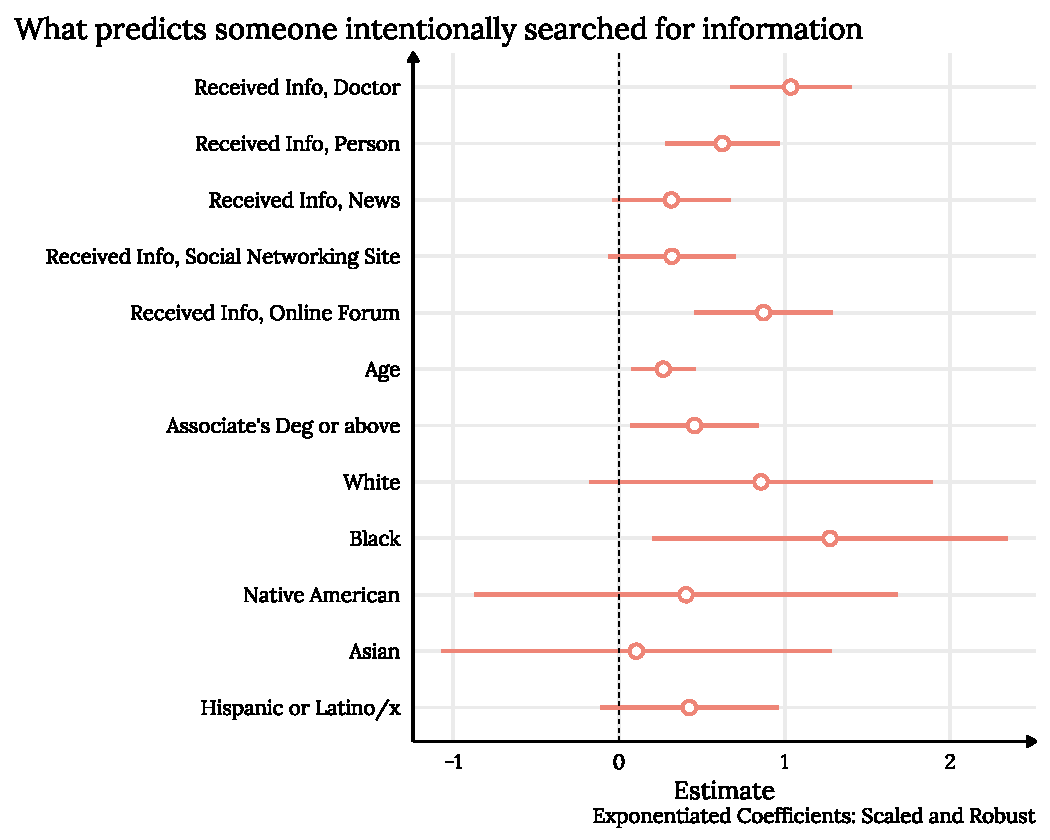
\includegraphics[width=0.8\linewidth]{figs/paper2/plot-model-1-1}}
\caption{Plot of Coefficients, Model 1}\label{fig:plot-model-1}
\end{figure}

Table \ref{tab:table-model-1} provides the results of my logistic regression
analysis predicting whether someone sought information about Covid-19. These
initial results suggest similar results for each vehicle of information
delivery: each mode of receiving information whether from a doctor, a person,
the news, a social networking site, or an online forum, all increase the odds of
seeking out information. For example, respondents who had received information
from a doctor or other medical professional were 2.82
(relative odds ratio = \(exp(\beta k)\), \emph{p} \textless{} 0.001) times more likely to seek
out information over someone who hadn't. Similarly, respondents who had received
information from `a person like friend, neighbor, or family member that {[}they{]} know'
were 1.87
( \emph{p} \textless{} 0.001) times more likely to seek out information over someone who hadn't
received information from a person like that. Interesting, those who had
received information from an online discussion group, listserve, or other online
forum including a Facebook group or subreddit were
2.39 ( \emph{p} \textless{} 0.001)
times more likely to search out more information than someone who hadn't. While
most demographic variables don't seem to have a strong effect on whether someone
sought out information about the Covid-19 vaccine, a few key variables had strong
associations. Age, for instance, is associated with seeking information; every
additional year of age a person holds they are
3\%
more likely to search for information, possibly indicating a generational effect
of information seeking patterns ( \emph{p} \textless{} 0.01). Additionally, those who were more
educated, that is those with an associate's degree or higher, were
1.58
more likely to seek additional information than those without the degree
( \emph{p} \textless{} 0.05). And finally, there is evidence to suggest that the Black or
African American sample was more likely to seek out information, specifically:
Blacks were 3.58 times more likely
to seek out information over non-Blacks ( \emph{p} \textless{} 0.05). Figure \ref{fig:plot-model-1} illustrates
the relationship between the coefficients and information seeking.

\hypertarget{information-search-vehicles}{%
\subsection{Information Search Vehicles}\label{information-search-vehicles}}

\begin{table}[ht]

\caption{\label{tab:model-2-phi}Phi Coefficient ($\phi$) of binary association between each Information Search Vehicle}
\centering
\begin{tabular}{p{0.25\linewidth} p{0.10\linewidth} p{0.08\linewidth} p{0.12\linewidth} p{0.15\linewidth} p{0.12\linewidth}}\toprule
 & Person & Dr & Online Forum & SNS & Online Search \\\toprule
Person & \- &  0.28& 0.172& 0.275& 0.216 \\
Dr & \- &  \- &  0.192 & 0.152 & 0.098 \\
Online Forum& \- &  \- &  \- &  0.371& -0.073 \\
SNS & \- &  \- &  \- &  \- &  0.057 \\
Online Search& \- &  \- &  \- &  \- &  \\
\bottomrule
\multicolumn{6}{l}{\rule{0pt}{1em}Notes: SNS = Social Networking Site}\\

\end{tabular}
\end{table}

To further investigate how people search for information, I asked those who had
sought information out intentionally, ``How did you look for information about
the Covid-19 vaccine?'' Because respondents could select as many responses as
applicable, each response is recorded as a dichotomous variable. Table
\ref{tab:table-1-desc} reveals differences in the prevalence of usage of the
various information seeking vehicles: Around 40\% of the sample has inquired for
information from a doctor, a person, or using online search tool (44\%, 42\%, 41\%) while my
respondents used vehicles like online forums (27\%) and social networking sites (18\%)
to seek out information at significantly lower rates. To investigate how each
Information Search Vehicle are related to each other using the Phi Coefficient
(\(\\phi\)) of binary association between each Information Search Vehicle pair.
The Phi coefficient can be interpreted like a correlation coefficient, with
numbers closer to -1 or positive one indicating a very strong relationship
(Warrens 2008). Table \ref{tab:model-2-phi} shows the results of these
coefficients. Out of the five information search vehicles investigated, there is
evidence that the vehicles are distinctly different concepts because most
coefficients fall under 0.3, the general rule of thumb for correlation
coefficients to indicate a relationship. There does seem to be a relationship
between Online Forums and Social Networking Sites, possibly due to an
individual's propensity to use online networks over in-person networks. These
coefficients indicate a weak relationship between any two vehicles of
information search and that respondents in my sample utilize each of these a
little bit differently.

\begin{table}[!h]

\caption{\label{tab:table-model-2}What predicts someone intentionally searched for information, by vehicle of information search}
\centering
\resizebox{\linewidth}{!}{
\begin{tabular}[t]{llllll}
\toprule
\multicolumn{1}{c}{ } & \multicolumn{5}{c}{Dependent Variable} \\
\cmidrule(l{3pt}r{3pt}){2-6}
  & Doctor & Person & Online Forum & Social Networking Site & Online Search\\
\midrule
\cellcolor{gray!6}{Received Info, Doctor} & \cellcolor{gray!6}{\num{1.942}***} & \cellcolor{gray!6}{\num{1.124}***} & \cellcolor{gray!6}{\num{0.181}} & \cellcolor{gray!6}{\num{0.540}**} & \cellcolor{gray!6}{\num{0.430}**}\\
Received Info, Person & \num{0.800}*** & \num{1.199}*** & \num{0.728}*** & \num{0.281} & \num{0.365}*\\
\cellcolor{gray!6}{Received Info, News} & \cellcolor{gray!6}{\num{0.437}**} & \cellcolor{gray!6}{\num{0.100}} & \cellcolor{gray!6}{\num{0.359}*} & \cellcolor{gray!6}{\num{0.514}*} & \cellcolor{gray!6}{\num{1.091}***}\\
Received Info, Social Networking Site & \num{-0.130} & \num{0.437}** & \num{-0.603}** & \num{0.731}*** & \num{1.272}***\\
\cellcolor{gray!6}{Received Info, Online Forum} & \cellcolor{gray!6}{\num{0.412}*} & \cellcolor{gray!6}{\num{0.263}+} & \cellcolor{gray!6}{\num{1.266}***} & \cellcolor{gray!6}{\num{0.974}***} & \cellcolor{gray!6}{\num{0.695}***}\\
Age & \num{0.002} & \num{0.001} & \num{-0.007} & \num{-0.003} & \num{0.029}***\\
\cellcolor{gray!6}{Associate's Deg or above} & \cellcolor{gray!6}{\num{0.542}**} & \cellcolor{gray!6}{\num{0.154}} & \cellcolor{gray!6}{\num{1.086}***} & \cellcolor{gray!6}{\num{1.344}***} & \cellcolor{gray!6}{\num{-0.952}***}\\
White & \num{0.631} & \num{0.245} & \num{0.009} & \num{0.559} & \num{0.012}\\
\cellcolor{gray!6}{Black} & \cellcolor{gray!6}{\num{0.366}} & \cellcolor{gray!6}{\num{0.208}} & \cellcolor{gray!6}{\num{0.608}} & \cellcolor{gray!6}{\num{0.646}} & \cellcolor{gray!6}{\num{0.357}}\\
Native American & \num{0.309} & \num{-0.696} & \num{0.209} & \num{0.762} & \num{-0.831}\\
\cellcolor{gray!6}{Asian} & \cellcolor{gray!6}{\num{-0.294}} & \cellcolor{gray!6}{\num{-0.566}} & \cellcolor{gray!6}{\num{-2.496}**} & \cellcolor{gray!6}{\num{-0.568}} & \cellcolor{gray!6}{\num{0.634}}\\
Hispanic or Latino/x & \num{0.324} & \num{0.116} & \num{0.529}* & \num{0.632}** & \num{-0.585}*\\
\cellcolor{gray!6}{Num.Obs.} & \cellcolor{gray!6}{\num{948}} & \cellcolor{gray!6}{\num{948}} & \cellcolor{gray!6}{\num{948}} & \cellcolor{gray!6}{\num{948}} & \cellcolor{gray!6}{\num{948}}\\
\midrule
$R_{McFadden}^2$ & \num{0.193} & \num{0.121} & \num{0.145} & \num{0.154} & \num{0.221}\\
\cellcolor{gray!6}{BIC} & \cellcolor{gray!6}{\num{1152.2}} & \cellcolor{gray!6}{\num{1237.6}} & \cellcolor{gray!6}{\num{1048.0}} & \cellcolor{gray!6}{\num{864.8}} & \cellcolor{gray!6}{\num{1104.6}}\\
Log.Lik. & \num{-524.709} & \num{-567.376} & \num{-472.576} & \num{-380.971} & \num{-500.907}\\
\bottomrule
\multicolumn{6}{l}{\rule{0pt}{1em}* p $<$ .05. ** p $<$ .01. *** p $<$ .001 (two-tailed test).}\\
\multicolumn{6}{l}{\rule{0pt}{1em}Raw, Unexponentiated Coefficients}\\
\end{tabular}}
\end{table}


Results of each logistic regression are displayed in Table \ref{tab:table-model-2}.
Modeling each response as a separate formula is useful for interpretation, but
there are important caveats: because each logistic regression is on a different
scale, one must not compare the magnitude of coefficients between models. We
can, however, use the direction and significance of the coefficients to draw
conclusions about these different forms of information search vehicles.

The first model in Table \ref{tab:table-model-2} predicts whether a
respondent sought information intentionally about Covid-19 vaccinations by
asking their doctor or another health professional. First and foremost, I find
that those who received information about Covid-19 vaccinations were
6.97 times
more likely to seek out more information from their doctor than those who had
not ( \emph{p} \textless{} 0.001). However, receiving information from other vehicles also
increased the odds of seeking out information from medical professions. Those who
received information from a person like a friend or a relative were
2.23 times more likely to ask their doctor ( \emph{p} \textless{} 0.001), while those who received
information from the news or television were 1.55 times more likely ( \emph{p} \textless{} 0.01). I also find that those who received information from an online forum like a subreddit were 51\% more likely to ask their doctors than those who hadn't ( \emph{p} \textless{} 0.05). Finally, respondents with an associate's degree or higher were 72\%
more likely to ask their doctor for information on the Covid-19 vaccinations
than those who held less education ( \emph{p} \textless{} 0.01).

The second model predicts whether a respondent sought information about
Covid-19 vaccinations by asking a person like friend, neighbor, or family member
that they know. Only three coefficients in this model were significant and help
us draw any conclusions on who is most likely to activate their personal social
network for informational support. In this study, I find that receiving
information about the vaccine from a doctor, their personal network, or a social
networking site is associated with seeking out more information. Those who
received information from a doctor or other medical professional were 3.08
times more likely to seek information from a person like a friend ( \emph{p} \textless{} 0.001).
Moreover, it seems that receiving information from your personal social network,
like a friend or relative, is associated with seeking information from those
same people; in fact, I find that those who did are 3.32 more
likely to do so ( \emph{p} \textless{} 0.001). Finally, the respondents who received information
about the vaccine on a social networking site were 55\%
more likely to seek information from their personal network than those who hadn't
( \emph{p} \textless{} 0.01). The unexpected result of this model is that very few factors predict
personal social network activation, and this model has the lowest McFadden's R\^{}2,
indicating possible omitted variables.

I also wanted to see what was associated with posting in an online discussion
group, listserve, or other online forum like a Facebook Group or Subreddit about
Covid-19 vaccinations. This is conceptually different that posting a query on a
social networking site like Facebook or twitter where identities are involved,
but is theoretically more {[}costly?{]}{[}friction?{]} than searching on an internet
search engine. I found that having received information about the vaccine from
your personal social network (like a friend or relative), the news, or an online
forum was associated with higher odds of querying an online forum. Specifically,
receiving information from your personal network is associated with 2.07
higher odds ( \emph{p} \textless{} 0.001), from news or television media with 1.43 higher odds ( \emph{p} \textless{} 0.05), and receiving information on an online forum associated with 3.55
higher odds ( \emph{p} \textless{} 0.001). Moreover, I found that those with an associate's
degree or above were 2.96 times 
more likely to search for information on an online forum ( \emph{p} \textless{} 0.001). Finally,
I found a racial-ethnic with Hispanic-Latinos; I found that they were about 70\%
more likely to query an online forum than non-Hispanics ( \emph{p} \textless{} 0.05). However,
there were also a few variables that lowered the odds of posting in an online
discussion group. First, those who had received information from a social networking site were 45\%
less likely to query a forum than those who hadn't (relative odds ratio =
\(1 - exp(\beta k)\), \emph{p} \textless{} 0.01). Moreover, I find more ethnoracial effects:
Respondents who claimed Asian ancestry were 92\%
less likely to query online forum ( \emph{p} \textless{} 0.01).

The fourth model predicts whether an individual sought information about
Covid-19 vaccinations through posted queries on a social networking site such
as Facebook timeline, Twitter status update, or LinkedIn. Receiving information
about Covid-19 seems to be quite related to posting on social media. Those who
received information from their doctor's had 1.72
higher odds of posting on a social networking site ( \emph{p} \textless{} 0.01), while those
who received their information from tv/news had 1.67 higher odds ( \emph{p} \textless{} 0.05).
Furthermore, those who received information on social networking sites were more
likely to post queries on social networking sites (\(\beta\) = 2.08, \emph{p} \textless{} 0.001).
The respondents in our sample who received information on online forums had 2.65
higher odds of posting queries on their social networking platforms ( \emph{p} \textless{} 0.001).
I found a relationship between education and posting on social networking sites
as well; specifically, those with an Associate's degree or above were 3.83 times more likely to post vaccination
queries on social networking sites than those with lower education ( \emph{p} \textless{} 0.001).
Finally, I find that Hispanic-Latinos were 88\%
more likely to ask their connections on a social networking site about the
Covid-19 vaccinations than non-Hispanics ( \emph{p} \textless{} 0.01).

Searching for information using an online search engine such as Google or Bing
is theoretically the search vehicle with the least amount of social or cognitive
friction. Our descriptive statistics showed that not everyone used this vehicle,
with only 41\% of our sample (See Table \ref{tab:table-1-desc}) having sought
information about the Covid-19 vaccines using online search engines. My model
reveals interesting patterns to help explain the variation. As with previous
models, receiving information of any kind increase the odds of online search,
though to varying magnitudes (Doctor: 1.54 odds; Person: 1.44 odds; News or Television: 2.98 odds; Social Networking Site: 3.57 odds; Online Forum: 2 odds). I also find that older respondents were more likely to search online, with each
addition year aged to yield 3\%
higher odds of searching online ( \emph{p} \textless{} 0.001). The most interesting variations
come from what decreases the odds of online search. First, those with an
Associate's degree or higher were 61\%
less likely to search online for questions about Covid-19 than those with less
educational attainment ( \emph{p} \textless{} 0.001). In addition, I find that Hispanic-Latinos
had 44\% lower odds of searching online than non-Hispanics ( \emph{p} \textless{} 0.05).

\hypertarget{vaccination-views}{%
\subsection{Vaccination Views}\label{vaccination-views}}

\begin{table}[!h]

\caption{\label{tab:table-model-3}Does receiving or searching for information predict vaccination status?}
\centering
\begin{tabular}[t]{lc}
\toprule
  & Model 1\\
\midrule
\cellcolor{gray!6}{Received Info, Doctor} & \cellcolor{gray!6}{\num{1.049}*** (\num{0.301})}\\
Received Info, Person & \num{-0.206} (\num{0.242})\\
\cellcolor{gray!6}{Received Info, News} & \cellcolor{gray!6}{\num{0.108} (\num{0.247})}\\
Received Info, Social Networking Site & \num{-0.794}*** (\num{0.240})\\
\cellcolor{gray!6}{Received Info, Online Forum} & \cellcolor{gray!6}{\num{-0.321} (\num{0.248})}\\
Sought Info, Doctor & \num{1.386}*** (\num{0.341})\\
\cellcolor{gray!6}{Sought Info, Person} & \cellcolor{gray!6}{\num{0.570}* (\num{0.285})}\\
Sought Info, Social Networking Site & \num{0.710} (\num{0.466})\\
\cellcolor{gray!6}{Sought Info, Online Forum} & \cellcolor{gray!6}{\num{0.354} (\num{0.342})}\\
Sought Info, Online Search & \num{0.085} (\num{0.260})\\
\cellcolor{gray!6}{Age} & \cellcolor{gray!6}{\num{-0.018}+ (\num{0.011})}\\
Associate's Deg or above & \num{1.281}*** (\num{0.234})\\
\cellcolor{gray!6}{White} & \cellcolor{gray!6}{\num{1.122} (\num{0.767})}\\
Black & \num{0.808} (\num{0.799})\\
\cellcolor{gray!6}{Native American} & \cellcolor{gray!6}{\num{0.126} (\num{0.829})}\\
Asian & \num{1.555}+ (\num{0.918})\\
\cellcolor{gray!6}{Hispanic or Latino/x} & \cellcolor{gray!6}{\num{1.039}* (\num{0.505})}\\
Num.Obs. & \num{936}\\
\midrule
\cellcolor{gray!6}{$R_{McFadden}^2$} & \cellcolor{gray!6}{\num{0.261}}\\
BIC & \num{669.2}\\
\cellcolor{gray!6}{Log.Lik.} & \cellcolor{gray!6}{\num{-266.187}}\\
\bottomrule
\multicolumn{2}{l}{\rule{0pt}{1em}* p $<$ .05. ** p $<$ .01. *** p $<$ .001 (two-tailed test).}\\
\multicolumn{2}{l}{\rule{0pt}{1em}Raw, Unexponentiated Coefficients}\\
\end{tabular}
\end{table}

Finally, in Table \ref{tab:table-model-3}, I investigate whether there is a
relationship between information receiving and information seeking behaviors and
the choice to get vaccinated against Covid-19 through a logistic regression
model predicting Vaccination Outlook. I find that receiving information from a
doctor or other medical profession is associated with
2.85 odds of receiving
a Covid-19 vaccinated ( \emph{p} \textless{} 0.001) and that seeking information from a doctor
also increases the odds of vaccination by
4 ( \emph{p} \textless{} 0.001).
I find that my respondents who received information on a social networking site
like Facebook or Twitter about the vaccines were 55\%
\textbf{less likely} to get vaccinated than those who received no information through
that vehicle ( \emph{p} \textless{} 0.001). However, I did find that those who reached out to
family or friends with their concerns were
77\% more likely to become vaccinated ( \emph{p} \textless{} 0.05). Furthermore, my respondents who held an
Associate's degree or above had 3.6
higher odds of becoming immunized ( \emph{p} \textless{} 0.001). And finally, I found further
ethnoracial differences in my sample. I found that Hispanic-Latinos had
2.83 higher odds of vaccination
than non-Hispanics ( \emph{p} \textless{} 0.05) and that my Asian sample had
4.73 higher odds as well over
non-Asians ( \emph{p} = 0.09). See Figure \ref{fig:plot-model-3} for a visual
representation of how these different coefficients are related to vaccination outlook.

\begin{figure}
{\centering 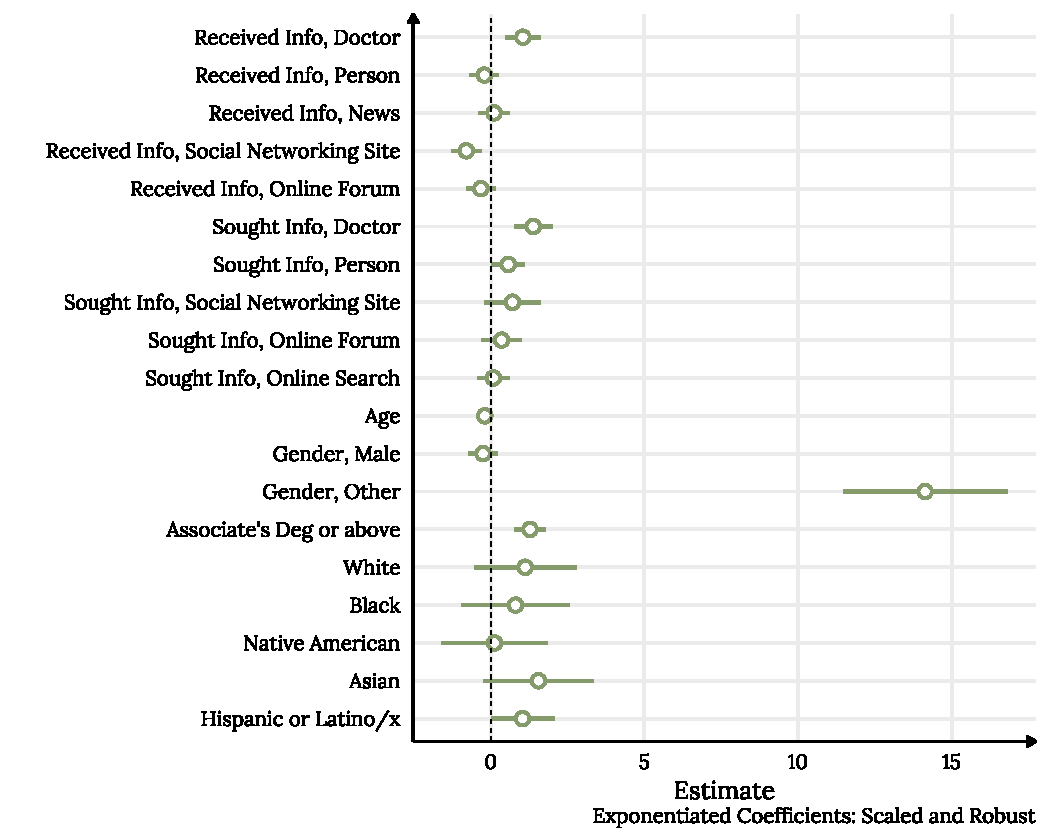
\includegraphics[width=0.8\linewidth]{figs/paper2/plot-model-3-1}}
\caption{Plot of Coefficients, Model 3}\label{fig:plot-model-3}
\end{figure}

\hypertarget{discussion}{%
\section{Discussion}\label{discussion}}

Previous research in Sociology and Infodemiology has greatly failed to
distinguish between the activation of information seeking behaviors online and
offline. In this paper, I aim to uncover just how different various methods of
information search are and begin a line of research inquiry that investigates
the factors associated with each different vehicle. Finally, I also aimed to
uncover how the different fountains of information and information search
vehicles hold real world consequences through their associations with Covid-19
vaccination rates and intentions.

I first find that receiving information about Covid-19 vaccinations from any
outlined source increases the likelihood of searching out more information. I
also find important demographic differences in the overall propensity to seek
out information. First, I find that the older a respondent is, the more likely
they are to seek out information about Covid-19 vaccinations, possibly
indicating a larger information need by elderly populations overall, or a more
pressing need to search for information about the Covid-19 vaccinations because
of the higher risk of hospitalizations that older populations face
\citep{turner_etal18}. Furthermore, I find that those who are college educated were
more likely to seek out information; for the most part this trend can be
observed in Table \ref{tab:table-model-2} as well. Human Capital Theory
\citep{mirowsky_ross98} may help to explain this finding; this theory claims that
higher education can provides the skills to gain health-related knowledge and
use this knowledge to be proactive in their own lives. Finally, I find that my
respondents who identified as Black were more likely to seek out further
information; this may be explained by the maltreatment that African Americans
have endured in the US healthcare system \citep{baileyStructuralRacismHealth2017}
which has led to major distrust of the medical establishment among the
population \citep{center2019, murray15, bronson2014don}.

Table \ref{tab:table-model-2} further demonstrated important takeaways about
how individuals seek information. First, I find that the different information
seeking vehicles queried in this survey are conceptually different and that the
utilization of different varies by demographic and supply 
% TODO (information fountain? \textasciitilde{} source of having receiving information). 
Overall, receiving information about
Covid-19 vaccination generally is associated with information seeking behaviors,
though there are key variations. First, if you received information from a
doctor, you were likely to search from information from a doctor; this may
indicate an already existing trusting relationship between patient and
healthcare provider but it may also indicate the healthcare provider taking
initiaive and emphasizing the importance of the vaccine or the survey respondent
seeking out information from an expert. Another important finding is that if you
received information from a Social Networking Site like Facebook or Twitter, you
were less likely to query Online Forums like Reddit or Facebook Groups; this may
be an example of Uses and Gratification Theory
\citep{blumlerUsesMassCommunications1974}, where the two online platforms may act as
substitute sources of information and those who were satisfied with the
information they received on a Social Networking Site didn't have the need to
seek out more information. Finally, the ethnoracial variations exhibited in
Table \ref{tab:table-model-2} likely demonstrate how cultural attitudes around
the trustworthiness of different sources of information affect the utilization
of different methods; for example, Asians seem are less likely to use online
forums than non-Asians while Hispanics are more likely to use them than
non-Hispanics. The internal variations between the different information search
vehicles hint at different user profiles and may have major repercussions on the
quality of information they find and who is exposed to poor quality information.

Given the rampant misinformation around Covid-19, her related vaccinations
\citep{pathakInfodemicsCOVID19Role2020, mottaHowRightLeaningMedia2020, shahsavariConspiracyTimeCorona2020}
and the slowed rate of vaccinations in the
United States, it is important to uncover what relationship the different
fountains of information and information search vehicles for Covid-19 vaccinations
are associated with compliance with public health recommendations. Table
\ref{tab:table-model-3} demonstrated just how these different fountains of
information and information search vehicles are associated with real world
consequences through Covid-19 vaccination rates and intentions. The first
takeaway is that receiving or seeking information from a doctor or other medical
profession was associated with higher likelihood of completed or planned vaccinations.
While blanket advice like ``Healthcare Providers should recommend the vaccine to
their patients'' would be ineffective because of the declining number of
Americans with a primary care doctor \citep{levine_etal20}, increasing trust in the
institution of medicine seems to remain a strong predictor of vaccinations.
A second major takeaway is that receiving information from a Social Networking
Site like Facebook timeline or Twitter status update was significantly
associated with lower vaccination rates. While we don't know what exact
information was absorbed on these platforms, the lower odds of vaccination
indicate that it was not positive. Much has been attempted between 2020 and 2022
to curb vaccine misinformation on these social networking platforms (see Bowman 2020 for an early example); however, I find evidence that these social
networking platforms nevertheless have a measurable negative impact. Finally,
this study also contributes to the conversation on ethnoracial and
educational differences in vaccine hesitancy. I find in my sample that
Hispanic-Latinos and Asians were more likely than non-Hispanics and non-Asians
to receive or plan to receive a vaccination against Covid-19 (Table
\ref{tab:table-model-3}). Research in this area has mixed results, with some
studies showcasing consistent findings to these \citep{bagasra_etal21,king_etal21},
while others show that Whites have the lowest levels of vaccine hesitancy and
many minorities are much more hesitant \citep{momplaisir_etal21, foxworth21}. My finding that college-educated respondents were more likely seek vaccination is largely consistent with the broader literature
\citep{khairat_etal22}, though again there are many variations depending on the vaccine
in question and study context \citep{siddiqui_etal13}.

\hypertarget{conclusion}{%
\section{Conclusion}\label{conclusion}}

Previous research has greatly failed to distinguish between the activation of
information seeking behaviors online and offline and largely focuses on the
information that is sent to consumers {[}push{]}, seeing people as passive receivers
of information. In this paper, I instead focus on individuals as active agents
in their search for information to begin a line of research inquiry that
investigates the factors associated with the various methods of information
search.

Given the large swaths of both misinformation and disinformation regarding
Covid-19 \citep{pathakInfodemicsCOVID19Role2020, mottaHowRightLeaningMedia2020, shahsavariConspiracyTimeCorona2020} and the measurable impacts this misinformation has had on pandemic-related health behaviors
\citep{loombaMeasuringImpactCOVID192021, greene_murphy21}, Covid-19 provides an ideal study to
investigate how we choose to search for information that affects both our own
lives and the lives of others.

This paper has provided several key findings that can be used to motivate policy
interventions for the Covid-19 vaccination campaigns and in the future for other
information campaigns. However, these findings are not to be taken out of the
context of their limitations. This paper is built off a small survey sample (
948) that was hosted online and anonymously through MTurk, a service
that provides people with micro-jobs. Because of how the website is set up,
respondents are incentivized to fill out surveys as quick as possible and there
were many responses that were poor quality and removed from the sample before
analysis. Because of this, there is no incentive for respondents to be honest in
these surveys. However, each of these limitations are often pointed to as
limitations of survey research as a whole. Even given these limitations,
the finding of this paper are interesting contributions to the literature.

Overall, this research project is important because the vehicles used in
information search impacts the information and quality of information found. By
looking at how individuals search, I aim to identified pain points and focus areas
for future interventions (receiving information online; ethnoracial variations) in the misinformation process.